% ****************************************************************************************************
\chapter{Simulating the Adoption Process of Platform as a Service Business Models}\label{ch:sfd}
% ****************************************************************************************************

Based on the above discussed qualitative model, within this chapter a quantitative model is developed in order to simulate the adoption process of \ac{PaaS} business models. As with the qualitative model, also for the hereafter introduced quantitative model the concept of system dynamics according to \citet{Sterman2000} and \citet{Sterman2001} is used. To be more specific, the overall qualitative model respectively \ac{CLD} (cf. Figure \ref{fig:cld_bp}) will be transferred into a quantitative model -- also known as \acf{SFD}. Hereby the third sub-research question will be answered, but also the main research question regarding high-leverage interventions and policies so as to achieve a high adoption rate.

% ****************************************************************************************************
\section{Stocks and Flows}\label{ch:sfd:sf}
% ****************************************************************************************************

The two central concepts of the system dynamics theory are stocks and flows as well as the feedback structure both of the system under investigation. Basically stocks accumulate flows over time. Moreover \textit{"they characterize the state of the system and generate the information upon which decisions and actions are based. Stocks give systems inertia and provide them with memory. Stocks create delays by accumulating the difference between the inflow to a process and its outflow. By decoupling rates of flow, stocks are the source of disequilibrium dynamics in system"} \citep[p. 192]{Sterman2000}.

\begin{figure}[tb]
	\centering
	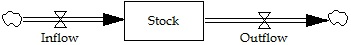
\includegraphics[width=0.5\textwidth]{gfx/sfd_basic}
	\caption[Stock and Flow Diagram -- Basics]{Stock and Flow Diagram -- Basics adapted from \citet[p. 194]{Sterman2000}}
	\label{fig:sfd_b}
\end{figure}

In Figure \ref{fig:sfd_b} the general structure of stocks and flows is illustrated. Every stock increases through one or more inflows. These flows can either come from outside the model, thus representing a model boundary (denoted as cloud) or from another stock, hence this kind of flow is an in- and outflow simultaneous (an outflow for stock A and an inflow for stock B). Through one or more outflows stocks decrease over time. These outflows can either represent a model boundary (denoted as cloud) or flow in another stock.

The size of a stock at any time is the accumulation of all its inflows less all its outflows. By using mathematical notation this states as follows: stocks integrate their flows. This leads to the following integral equation in line with \citet[p. 194]{Sterman2000} as shown in  Formula \ref{eq:int}:

\begin{equation}\label{eq:int}
		Stock(t) = \int\limits_{t_0}^t [Inflow(s) - Outflow(s)]ds + Stock(t_0)
\end{equation}

Whereas the $Inflow(s)$ respectively $Outflow(s)$ represent the flow at any time $s$ between the initial time $t_0$ and the current time $t$ and the initial size of the stock is denoted by $Stock(t_0)$. 

Another size of interest is the net rate of change of any stock, its derivative, is defined by the following differential equation in line with \citet[p. 194]{Sterman2000} as shown in Formula \ref{eq:dif}:

\begin{equation}\label{eq:dif}
		\frac{d(Stock)}{dt} = \mathit{Net~Change~in~Stock} = Inflow(t) - Outflow(t)
\end{equation}

Whereas the $Inflow(t)$ respectively $Ouflow(t)$ represent the flow at the current time $t$.

By applying the above described concept of stocks and flows onto the previous developed \ac{CLD} 11 crucial stocks in the domain of \ac{PaaS} business models were revealed (cf. Figure \ref{fig:sfd_cs}). The number of all stakeholders using the platform is denoted as customer base and increases through the inflow new customer. However, within this study the time horizon of investigating the platform adoption is rather considered in a short-time horizon. Due to this assumption, the stock customer base does not decrease through a corresponding outflow and simplifies the \ac{SFD} thereby. The remaining ten stocks are dedicated to the five earlier defined customer segments. Each customer segment is modeled as a stock of potential customers (denoted as potential <customer segment> \footnote{The wildcard \texttt{<customer segment>} represents the five earlier identified customer segments.}) and as a second stock of the customer population (denoted as <customer segment> population). These two stocks are linked through the flow new customers (denoted as new <customer segment>), whereas this flow decreases the stock potential <customer segment> and increases the stock <customer segment> population. As with the stock customer base, also for the 10 stocks dedicated to the five customer segments corresponding model boundaries have been defined. The <customer segment> population stock does not decrease through an outflow due to the rather short-time horizon -- comparable with the stock customer base. All five potential <customer segment> stocks are defined -- in regards to the initial size -- beforehand the platform adoption simulation and decrease over time through the corresponding outflows. These stocks can be defined in two different ways. First, by analyzing the market opportunities of the platform under investigation the numbers of potential customers for the five customer segments can be calculated and used for the simulation. And second, the simulation can be run using relative values ($0\%$ - $100\%$) and thereby indicating that at any time $x\%$ of the customer segment (this holds obvious for all customer segments) are using the platform.

The two above described flows -- new <customer segment> and new customer -- are influenced as follows. Literally the inflow new customer is the accumulation of the five customer segment inflows, denoted as new <customer segment> (cf. Formula \ref{eq:nc}).

NEW <CUSTOMER SEGMENT> INFLOWS influenced through
\begin{enumerate}
	\item	Innovators
	\item	Imitators
	\item	Adoption from CVP
\end{enumerate}

In Figure \ref{fig:sfd_cs} the above describe stock and flow structure for the \ac{PaaS} domain is illustrated.

\begin{figure}[tb]
	\centering
	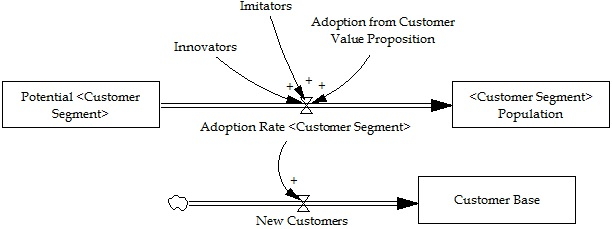
\includegraphics[width=0.8\textwidth]{gfx/sfd_customerSegment}
	\caption{Stock and Flow Diagram -- Generic PaaS Customer Segment}
	\label{fig:sfd_cs}
\end{figure}

% ****************************************************************************************************
\section{Model Foundations}\label{ch:sfd:mf}
% ****************************************************************************************************
In the following the model foundations are introduced which are necessary so as to simulate the platform adoption. Due to the fact that within the subsequent pages quite a few acronyms are used they are briefly listed in Table \ref{tab:acro} for reasons of clarity and comprehensibility.

\begin{table}[t]
	\centering
	\begin{tabular}{ll}
			\toprule 
			\footnotesize \textbf{Acronym} & \footnotesize \textbf{Meaning}	 \\ \midrule
			\footnotesize \acs{AR} & \footnotesize \acl{AR} \\ 
			\footnotesize \acs{PoP} & \footnotesize \acl{PoP}\\ 
			\footnotesize \acs{PoAaC} & \footnotesize \acl{PoAaC}\\ 
			\footnotesize \acs{UB} & \footnotesize \acl{UB} \\
			\footnotesize \acs{LB} & \footnotesize \acl{LB}\\ \midrule
			\footnotesize \acs{ITS} & \footnotesize \acl{ITS}\\
			\footnotesize \acs{SI} & \footnotesize \acl{SI}\\
			\footnotesize \acs{ISV} & \footnotesize \acl{ISV}\\
			\footnotesize \acs{PC} & \footnotesize \acl{PC}\\
			\footnotesize \acs{AC} & \footnotesize \acl{AC}\\ 
			\footnotesize \acs{CS} & \footnotesize \acl{CS}\\ \midrule
			\footnotesize \acs{GOV} & \footnotesize \acl{GOV}\\
			\footnotesize \acs{TS} & \footnotesize \acl{TS}\\
			\footnotesize \acs{AS} & \footnotesize \acl{AS}\\
			\footnotesize \acs{CVP} & \footnotesize \acl{CVP}\\ \midrule
			\footnotesize \acs{PI} & \footnotesize \acl{PI}\\
			\footnotesize \acs{PM} & \footnotesize \acl{PM}\\
			\footnotesize \acs{MP} & \footnotesize \acl{MP}\\ \bottomrule
	\end{tabular}
	\caption{Acronyms}
	\label{tab:acro}
\end{table}

As mentioned above, the flow $New~Customer(t)$ is the accumulation of the five customer segment inflows $New~CS(t)$ at any time $t$:

\begin{equation}\label{eq:nc}
	\mathit{New~Customer(t)} = \sum{\mathit{New~CS(t)}}
\end{equation}

The corresponding stock $Customer~Base(t)$ is simply the initial stock size $\mathit{Customer~Base(t_0)}$ increased by the inflow $New Customer(s)$:

\begin{equation}\label{eq:cb}
	\mathit{Customer~Base(t)} = \int\limits_{t_0}^t \mathit{[New~Customers(s)]ds} + \mathit{Customer~Base(t_0)}
\end{equation}

By using the stock $Customer~Base(t)$, the overall market penetration $MP_{Overall}(t)$ can be calculated. Due to the model simplifications, this value is the relation of the $Customer~Base(t)$ to the sum of all current ($Customer~Base(t)$) as well as potential ($Potential~CS$) customers:

\begin{equation}\label{eq:mpo}
	MP_{Overall}(t) = \frac{\mathit{Customer~Base(t)}}{\mathit{Customer~Base(t)} + \sum \mathit{Potential~CS(t)}} \in [0.0,1.0]
\end{equation}

Within Section \ref{ch:sfd:mv} and \ref{ch:sfd:mp} the model variables as well as parameters which are used in this model are introduced. These values need to be mapped to certain intervals so as to adjust the model dynamics. In order to map the values of the function $f(s) \in [a_1,a_2]$ to the desired interval $[b_1,b_2]$, the following generic linear transformation function is used:

\begin{equation}\label{eq:lt}
	f(t) = b_{1} + \frac{(s-a_1)(b_2-b_1)}{(a_2-a_1)} \in [b_1,b_2]
\end{equation}

In the particaular case of mapping the function $f(s) \in [0,1]$ to the interval $[b_1,b_2]$, the Formula \ref{eq:lt} can be simplified as follows:

\begin{equation}\label{eq:lts}
	f(t) = b_{1} + s (b_{2}-b_{1}) \in [b_{1},b_{2}].
\end{equation}

For the following five formulas this two linear transformation -- as appropriate simplified -- are used in order to map the corresponding functions to the desired intervals.

During the investigation of \ac{PaaS} business models, the difference between the pursued governance model have been noticed and considered in the classification scheme as well as \ac{CLD}. In the quantitative model, the value of the governance is considered unalterable due to the short-time horizon as well as to the assumption that \ac{PaaS} providers' will not change their governance model basically new. Therefore the initial governance model value $GOV(t_0)$ is just mapped into the corresponding interval -- between the lower $LB_{GOV}$ and upper boundary $UP_{GOV}$ -- by applying the simplified transformation function as shown in Formula \ref{eq:lts}:

\begin{equation}\label{eq:gov}
	GOV(t) = LB_{GOV} + GOV(t_0) * (UB_{GOV} - LB_{GOV}) \in [LB_{GOV},UB_{GOV}]
\end{equation}

Within the overall \ac{CLD} it was reasoned that an increase in the customer base will increase the revenue above what it would otherwise have been. Furthermore, through the increased revenue the platform investments will increase subsequent and finally resulting in increased platform improvements. However, in the \ac{SFD} this set of facts is simplified for reasons of clarity and comprehensibility. In order to take the quantitative model understandable although its complexity and to avoid adding too many external variables -- assumptions -- to this model, for the variable  platform improvements $PI(t)$ the value of the variable $MP_{Overall}$ (cf. Formula \ref{eq:mpo}) is simply mapped to the desired platform improvements interval (cf. Formula \ref{eq:lts}). Behind this simplification was the idea that an increased customer base will finally lead to higher platform improvements:

\begin{equation}\label{eq:pi}
	PI(t) = LB_{PI} + MP_{Overall}(t) * (UB_{PI} - LB_{PI}) \in [LB_{PI},UB_{PI}]
\end{equation}

The next two general values -- technical scope as well as additional services -- are further influencing factors which have been revealed and modeled previously. In contrast to the governance model, for this two factors it is considered that they improve over time through the variable platform improvements $PI(t)$ as calculated in Formula \ref{eq:pi}. Hence for any time $t$ the actually value for both is calculated by using the corresponding value of the last time step $t-1$ ($TS(t-1)$ respectively $ AS(t-1)$) and multiplying with the current platform improvements $PI(t)$. This intermediate value is then mapped to the desired interval. Due to specific intervals for this two variables, the denominator of the Formulas \ref{eq:ts} and \ref{eq:as} is equal to the upper boundary of the platform improvements $UB_{PI}$\footnote{Values for $TS(t_0)$ respectively $AS(t_0)$ are within the interval $[0.0,1.0]$ and for $PI(t)$ within the interval $[1.0,2.0]$ (cf. Section \ref{ch:sfd:mv} and \ref{ch:sfd:mp}). Thus the intermediate results ($TS(t-1)*PI(t)$ respectively $AS(t-1) *PI(t)$) are within the interval $[0.0,2.0]$ which represents the interval $[a_1,a_2]$ from Formula \ref{eq:lt}. Consequently the denominator for this linear transformation function is $2.0$ ($a_2 - a_1 = 2.0 - 0.0 = 2.0$), equals to $UB_{PI}$. This holds as long as $LB_{TS}$ respectively $LB_{AS}$ is equals to $0.0$.}:

\begin{equation}\label{eq:ts}
	TS(t) = LB_{TS} +  \frac{(TS(t_0) * PI(t)) * (UB_{TS} - LB_{TS})}{UB_{PI}} \in [LB_{TS},UB_{TS}]
\end{equation}

\begin{equation}\label{eq:as}
	AS(t) = LB_{AS} +  \frac{(AS(t_0) * PI(t)) * (UB_{AS} - LB_{AS})}{UB_{PI}} \in [LB_{AS},UB_{AS}]
\end{equation} 

Finally, the variable platform modules -- applications, services, components, or add-ons -- represent the last model foundation. As written above, platform modules are developed and deployed by complementors -- \acp{ISV} and \ac{IT} Startups -- and thus the values of the market penetration of these two customer segments ($MP_{ISV}(t)$ cf. Formula \ref{eq:mp:isv} respectively $MP_{ITS}(t)$ cf. Formula \ref{eq:mp:its}) are used in order to calculate the value of the platform modules. This approach was chosen again so as to avoid too many additional assumption -- parameter, variables, and the like. Therefore the two market penetration values are simply added and mapped to the desired interval by using the linear transformation formula (cf. Formula \ref{eq:lt}). In this particular case, the denominator of the Formula \ref{eq:pm} is equals to the sum of $UB_{ISV}$ and $UB_{ITS}$\footnote{Values for $MP_{ISV}(t)$ respectively $MP_{ITS}(t)$ are within the interval [0.0,1.0] (cf. Section \ref{ch:sfd:mp}). Thus the addition of $MP_{ISV}(t) + MP_{ITS}(t)$ results in the interval $[0.0,2.0]$ which represents the interval $[a_1,2_2]$ from Formula \ref{eq:lt}. Consequently the denominator for this linear transformation is $2.0$ ($a_2 - a_1 = 2.0 - 0.0 = 2.0$), equals to $UB_{ISV} + UB_{ITS}$.}:

\begin{eqnarray}\label{eq:pm}
	PM(t) = LB_{PM} + \frac{(MP_{ISV}(t) + MP_{ITS}(t)) * (UB_{PM} - LB_{PM})}{UB_{ISV} + UB_{ITS}} \nonumber \\ \in [LB_{PM},UB_{PM}]
\end{eqnarray}

% ****************************************************************************************************
\section{Customer-specific Formulas}\label{ch:sfd:csf}
% ****************************************************************************************************

% ****************************************************************************************************
\section{Model Variables}\label{ch:sfd:mv}
% ****************************************************************************************************

% ****************************************************************************************************
\section{Model Parameters}\label{ch:sfd:mp}
% ****************************************************************************************************

%Model Parameter
\newpage
\section{Model Parameter}
\begin{table}[tbh]
	\centering
	\begin{tabular}{ll}
			\toprule 
			Parameter & Interval resp. Values\\ \midrule
			PI & $[1,2]$ -> ($LB_{PI}$ = 1.0 and $UB_{PI}$ = 2.0) \\ 
			PM & $[1,2]$ -> ($LB_{PM}$ = 1.0 and $UB_{PM}$ = 2.0) \\ \midrule
			GOV & $[1,1.1]$ -> ($LB_{GOV}$ = 1.0 and $UB_{GOV}$ = 1.1) \\
			TS & $[1,1.1]$ -> ($LB_{TS}$ = 1.0 and $UB_{TS}$ = 1.1) \\
			AS & $[1,1.1]$ -> ($LB_{AS}$ = 1.0 and $UB_{AS}$ = 1.1) \\ \midrule
			$MP_{ITS}$ & $[0,1]$ -> ($LB_{ITS}$ = 0.0 and $UB_{ITS}$ = 1.0) \\
			$MP_{ISV}$ & $[0,1]$ -> ($LB_{ISV}$ = 0.0 and $UB_{ISV}$ = 1.0) \\
			$MP_{AC}$ & $[1,2]$ -> ($LB_{AC}$ = 1.0 and $UB_{AC}$ = 2.0) \\
			$MP_{SI_{PC}}$ & $[1,1.1]$ -> ($LB_{SI_{PC}}$ = 1.0 and $UB_{SI_{PC}}$ = 1.1) \\
			$MP_{SI_{AC}}$ & $[1,1.05]$ -> ($LB_{SI_{AC}}$ = 1.0 and $UB_{SI_{AC}}$ = 1.05) \\
			$MP_{PC}$ & $[1,1.2]$ -> ($LB_{PC}$ = 1.0 and $UB_{PC}$ = 1.2) \\ \bottomrule
	\end{tabular}
	\caption{Model Parameters}
	\label{tab:mpara}
\end{table}

%Model Variables
\newpage
\section{Model Variables}
\begin{table}[tbh]
	\centering
	\begin{tabular}{ll}
			\toprule 
			Variable & Interval\\ \midrule
			$GOV_i$ & $[0,1.0]$ \\
			$TS_i$ & $[0,1.0]$ \\
			$AS_i$ & $[0,1.0]$ \\ \midrule
			$CVP_{ITS_i}$ & $[0,0.1]$ \\
			$CVP_{ISV_i}$ & $[0,0.1]$ \\
			$CVP_{AC_i}$ & $[0,0.1]$ \\
			$CVP_{SI_i}$ & $[0,0.1]$ \\
			$CVP_{PC_i}$ & $[0,0.1]$ \\ \midrule
			$PoAaC_{ITS}$ & $[0,0.05]$ \\
			$PoAaC_{ISV}$ & $[0,0.05]$ \\
			$PoAaC_{AC}$ & $[0,0.05]$ \\
			$PoAaC_{SI}$ & $[0,0.05]$ \\
			$PoAaC_{PC}$ & $[0,0.05]$ \\ \bottomrule
	\end{tabular}
	\caption{Model Variables}
	\label{tab:mvar}
\end{table}

%ITS
\newpage
\section{ITS}

\begin{equation}
		CVP_{ITS} =  CVP_{ITS_{i}} * PI * MP_{AC} * MP_{PC}
\end{equation}

\begin{equation}
		AR_{ITS} = CVP_{ITS} * GOV * TS * AS		
\end{equation}

\begin{equation}
	PoP_{ITS} = \frac{\mathit{Population~ITS}}{\mathit{Population~ITS}+\mathit{Potential~ITS}}
\end{equation}

\begin{equation}
	\mathit{Adoption~from~AR_{ITS}} = PoP_{ITS} * AR_{ITS}
\end{equation}

\begin{equation}
	\mathit{Imitators~ITS} = PoP_{ITS} * PoAaC_{ITS}
\end{equation}

\begin{equation}
	\mathit{New~ITS} = \mathit{Adoption~from~AR_{ITS}} + \mathit{Imitators~ITS}
\end{equation}

\begin{equation}
	\mathit{Potential~ITS} = \mathit{Potential~ITS} - \mathit{New~ITS}
\end{equation}

\begin{equation}
	\mathit{Population~ITS} = \mathit{Population~ITS} + \mathit{New~ITS}
\end{equation}

\begin{equation}\label{eq:mp:its}
	MP_{ITS} = LB_{MP_{ITS}} + PoP_{ITS} * (UB_{MP_{ITS}} - LB_{MP_{ITS}})
\end{equation}

%ISV
\newpage
\section{ISV}

\begin{equation}
		CVP_{ISV} =  CVP_{ISV_{i}} * PI * MP_{AC} * MP_{PC}
\end{equation}

\begin{equation}
		AR_{ISV} = CVP_{ISV} * GOV * TS * AS		
\end{equation}

\begin{equation}
	PoP_{ISV} = \frac{\mathit{Population~ISV}}{\mathit{Population~ISV}+\mathit{Potential~ISV}}
\end{equation}

\begin{equation}
	\mathit{Adoption~from~AR_{ISV}} = PoP_{ISV} * AR_{ISV}
\end{equation}

\begin{equation}
	\mathit{Imitators~ISV} = PoP_{ISV} * PoAaC_{ISV}
\end{equation}

\begin{equation}
	\mathit{New~ISV} = \mathit{Adoption~from~AR_{ISV}} + \mathit{Imitators~ISV}
\end{equation}

\begin{equation}
	\mathit{Potential~ISV} = \mathit{Potential~ISV} - \mathit{New~ISV}
\end{equation}

\begin{equation}
	\mathit{Population~ISV} = \mathit{Population~ISV} + \mathit{New~ISV}
\end{equation}

\begin{equation}\label{eq:mp:isv}
	MP_{ISV} = LB_{MP_{ISV}} + PoP_{ISV} * (UB_{MP_{ISV}} - LB_{MP_{ISV}})
\end{equation}

%AC
\newpage
\section{AC}

\begin{equation}
		CVP_{AC} =  CVP_{AC_{i}} * PI * PM * MP_{SI_{AC}}
\end{equation}

\begin{equation}
		AR_{AC} = CVP_{AC} * GOV * TS * AS		
\end{equation}

\begin{equation}
	PoP_{AC} = \frac{\mathit{Population~AC}}{\mathit{Population~AC}+\mathit{Potential~AC}}
\end{equation}

\begin{equation}
	\mathit{Adoption~from~AR_{AC}} = PoP_{AC} * AR_{AC}
\end{equation}

\begin{equation}
	\mathit{Imitators~AC} = PoP_{AC} * PoAaC_{AC}
\end{equation}

\begin{equation}
	\mathit{New~AC} = \mathit{Adoption~from~AR_{AC}} + \mathit{Imitators~AC}
\end{equation}

\begin{equation}
	\mathit{Potential~AC} = \mathit{Potential~AC} - \mathit{New~AC}
\end{equation}

\begin{equation}
	\mathit{Population~AC} = \mathit{Population~AC} + \mathit{New~AC}
\end{equation}

\begin{equation}
	MP_{AC} = LB_{MP_{AC}} + PoP_{AC} * (UB_{MP_{AC}} - LB_{MP_{AC}})
\end{equation}

%SI
\newpage
\section{SI}

\begin{equation}
		CVP_{SI} =  CVP_{SI_{i}} * PI * PM * MP_{AC} * MP_{PC}
\end{equation}

\begin{equation}
		AR_{SI} = CVP_{SI} * GOV * TS * AS		
\end{equation}

\begin{equation}
	PoP_{SI} = \frac{\mathit{Population~SI}}{\mathit{Population~SI}+\mathit{Potential~SI}}
\end{equation}

\begin{equation}
	\mathit{Adoption~from~AR_{SI}} = PoP_{SI} * AR_{SI}
\end{equation}

\begin{equation}
	\mathit{Imitators~SI} = PoP_{SI} * PoAaC_{SI}
\end{equation}

\begin{equation}
	\mathit{New~SI} = \mathit{Adoption~from~AR_{SI}} + \mathit{Imitators~SI}
\end{equation}

\begin{equation}
	\mathit{Potential~SI} = \mathit{Potential~SI} - \mathit{New~SI}
\end{equation}

\begin{equation}
	\mathit{Population~SI} = \mathit{Population~SI} + \mathit{New~SI}
\end{equation}

\begin{equation}
	MP_{SI_{PC}} = LB_{MP_{SI_{PC}}} + PoP_{SI} * (UB_{MP_{SI_{PC}}} - LB_{MP_{SI_{PC}}})
\end{equation}

\begin{equation}
	MP_{SI_{AC}} = LB_{MP_{SI_{AC}}} + PoP_{SI} * (UB_{MP_{SI_{AC}}} - LB_{MP_{SI_{AC}}})
\end{equation}

%PC
\newpage
\section{PC}

\begin{equation}
		CVP_ {PC} =  CVP_{PC_{i}} * PI * PM * MP_{SI_{PC}}
\end{equation}

\begin{equation}
		AR_{PC} = CVP_{PC} * GOV * TS * AS		
\end{equation}

\begin{equation}
	PoP_{PC} = \frac{\mathit{Population~PC}}{\mathit{Population~PC}+\mathit{Potential~PC}}
\end{equation}

\begin{equation}
	\mathit{Adoption~from~AR_{PC}} = PoP_{PC} * AR_{PC}
\end{equation}

\begin{equation}
	\mathit{Imitators~PC} = PoP_{PC} * PoAaC_{PC}
\end{equation}

\begin{equation}
	\mathit{New~PC} = \mathit{Adoption~from~AR_{PC}} + \mathit{Imitators~PC}
\end{equation}

\begin{equation}
	\mathit{Potential~PC} = \mathit{Potential~PC} - \mathit{New~PC}
\end{equation}

\begin{equation}
	\mathit{Population~PC} = \mathit{Population~PC} + \mathit{New~PC}
\end{equation}

\begin{equation}
	MP_{PC} = LB_{MP_{PC}} + PoP_{PC} * (UB_{MP_{PC}} - LB_{MP_{PC}})
\end{equation}
